%!TEX root = ../../csuthesis_main.tex
\chapter{视觉目标跟踪模块设计}

\section{数据集采集机制与结构设计}

在视觉目标跟踪与意图分析的系统开发过程中,数据集的构建与管理至关重要。特别是在自动驾驶场景中,为了实现精准的模型训练、评估与算法验证,必须依赖具有真实感的动态交通数据以及结构化的标签体系。鉴于现实环境数据获取存在诸多限制,本文基于 Carla 仿真平台开发了一套自动化的数据采集与标注机制,结合传感器模拟输出与同步控制策略,生成涵盖图像、速度、位置、身份等信息的高质量标注样本集。

\subsection{采集流程设计}

系统在每次仿真运行过程中,自动采集模拟车载摄像头所捕获的图像帧,并实时提取当前帧中出现的其他车辆目标。通过调用 Carla 提供的车辆状态接口,可获取目标的三维位置和速度信息,并进一步通过变换矩阵将其投影至摄像头图像坐标系中,形成可用于目标检测任务的二维边界框。

为增强数据的多样性和实用性,系统设计了如下采集流程:

\textbf{(1)	图像获取:}定期(如每隔 5 帧)从主摄像头传感器中截取 RGB 图像;

\textbf{(2)	目标提取:}从当前帧中提取所有可见车辆,获取其三维边界框与速度;

\textbf{(3)	投影计算:}将三维框转换为图像平面坐标,形成二维检测框;

\textbf{(4)	追踪标记:}判断是否为当前正在追踪的目标,赋予唯一 ID;

\textbf{(5)	结果保存:}将图像帧以 JPG 格式保存,同时输出 JSON 格式的结构化标签文件。

该流程确保了采集数据具有高时效性与完整标签结构,满足后续目标检测、跟踪与行为识别等多任务需求。

\begin{figure}[H]
    \centering
    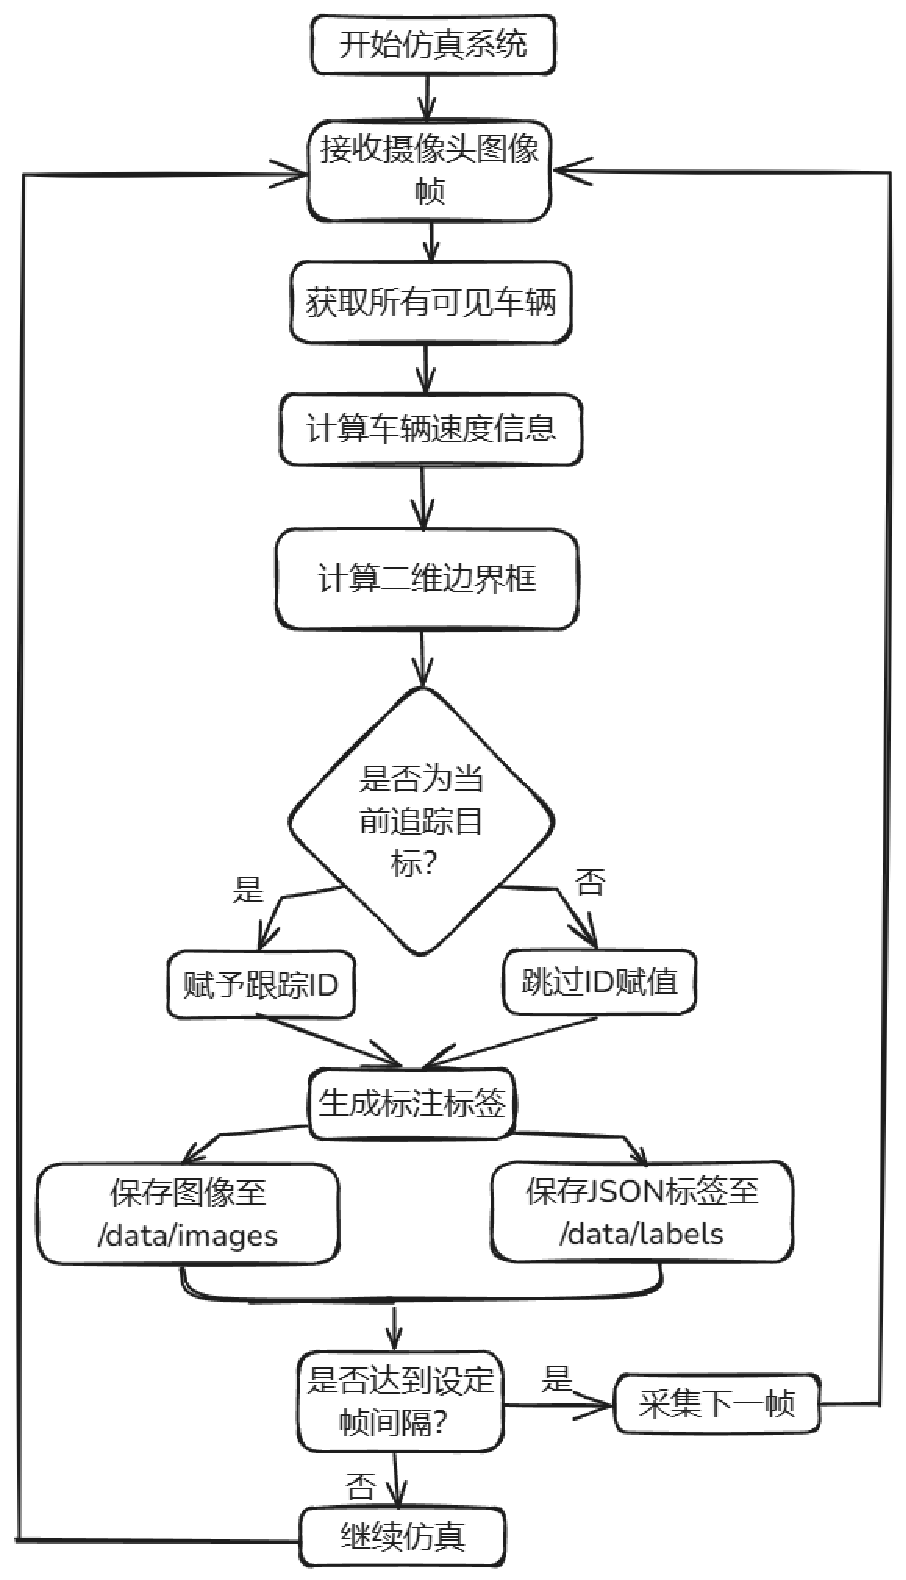
\includegraphics[width=0.8\textwidth]{images/图7 数据采集流程图.pdf}  % 引用转换后的 PDF 文件
    \caption{数据采集流程图}
    \label{fig:example_image}  % 可用于引用此图片
\end{figure}

\subsection{标注信息结构设计}

每个 JSON 标签文件对应一帧图像,包含该图像中所有检测到的车辆目标。标签信息以列表形式记录,每一项包含如下字段:

\textbf{bbox:}二维边界框左上角起 4 个顶点的图像坐标;

\textbf{speed\_m\_s:}目标瞬时速度(单位为米每秒);

\textbf{tracked\_id:}若目标被当前追踪模型识别并持续跟踪,则记录其分配 ID,否则为 null。

该结构兼容常用目标检测框架(如 YOLO、Faster R-CNN)与跟踪框架(如 DeepSORT、ByteTrack)所需数据格式,亦可拓展用于行为分析任务中的时序建模。

\begin{figure}[H]
    \centering
    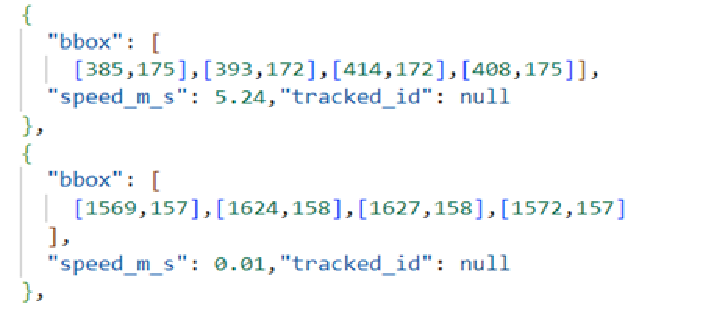
\includegraphics[width=0.8\textwidth]{images/图8 数据文件结构截图.pdf}  % 引用转换后的 PDF 文件
    \caption{数据文件结构截图}
    \label{fig:example_image}  % 可用于引用此图片
\end{figure}

\section{目标检测与跟踪模型设计}

\subsection{目标检测策略设计}

目标检测作为视觉感知系统的首要环节,是后续目标跟踪与意图分析的基础。为提升系统的整体运行效率与鲁棒性,本文在仿真环境中选用了一种基于物理建模的投影式目标检测方法,依托 Carla 平台提供的三维边界框与车辆状态信息,绕过传统深度学习模型的推理过程,实现了高精度、低延迟的目标检测策略。

在 Carla 中,每一个交通参与体(包括车辆、行人、自行车等)在生成时均自带三维边界框信息(Bounding Box),如下图4-3所示,该边界框由对象的局部中心点、长宽高(extent)及朝向参数共同定义,真实反映了目标的空间占用情况。这些边界框以局部坐标形式存在,需要经过变换才能映射到图像平面。具体而言,系统首先获取目标的边界框顶点坐标,然后将其从局部坐标系转换为世界坐标,再通过摄像头的变换矩阵投影至相机坐标系,最后利用相机的内参完成二维图像平面的投影,形成目标在图像中的二维边界框。

\begin{figure}[H]
    \centering
    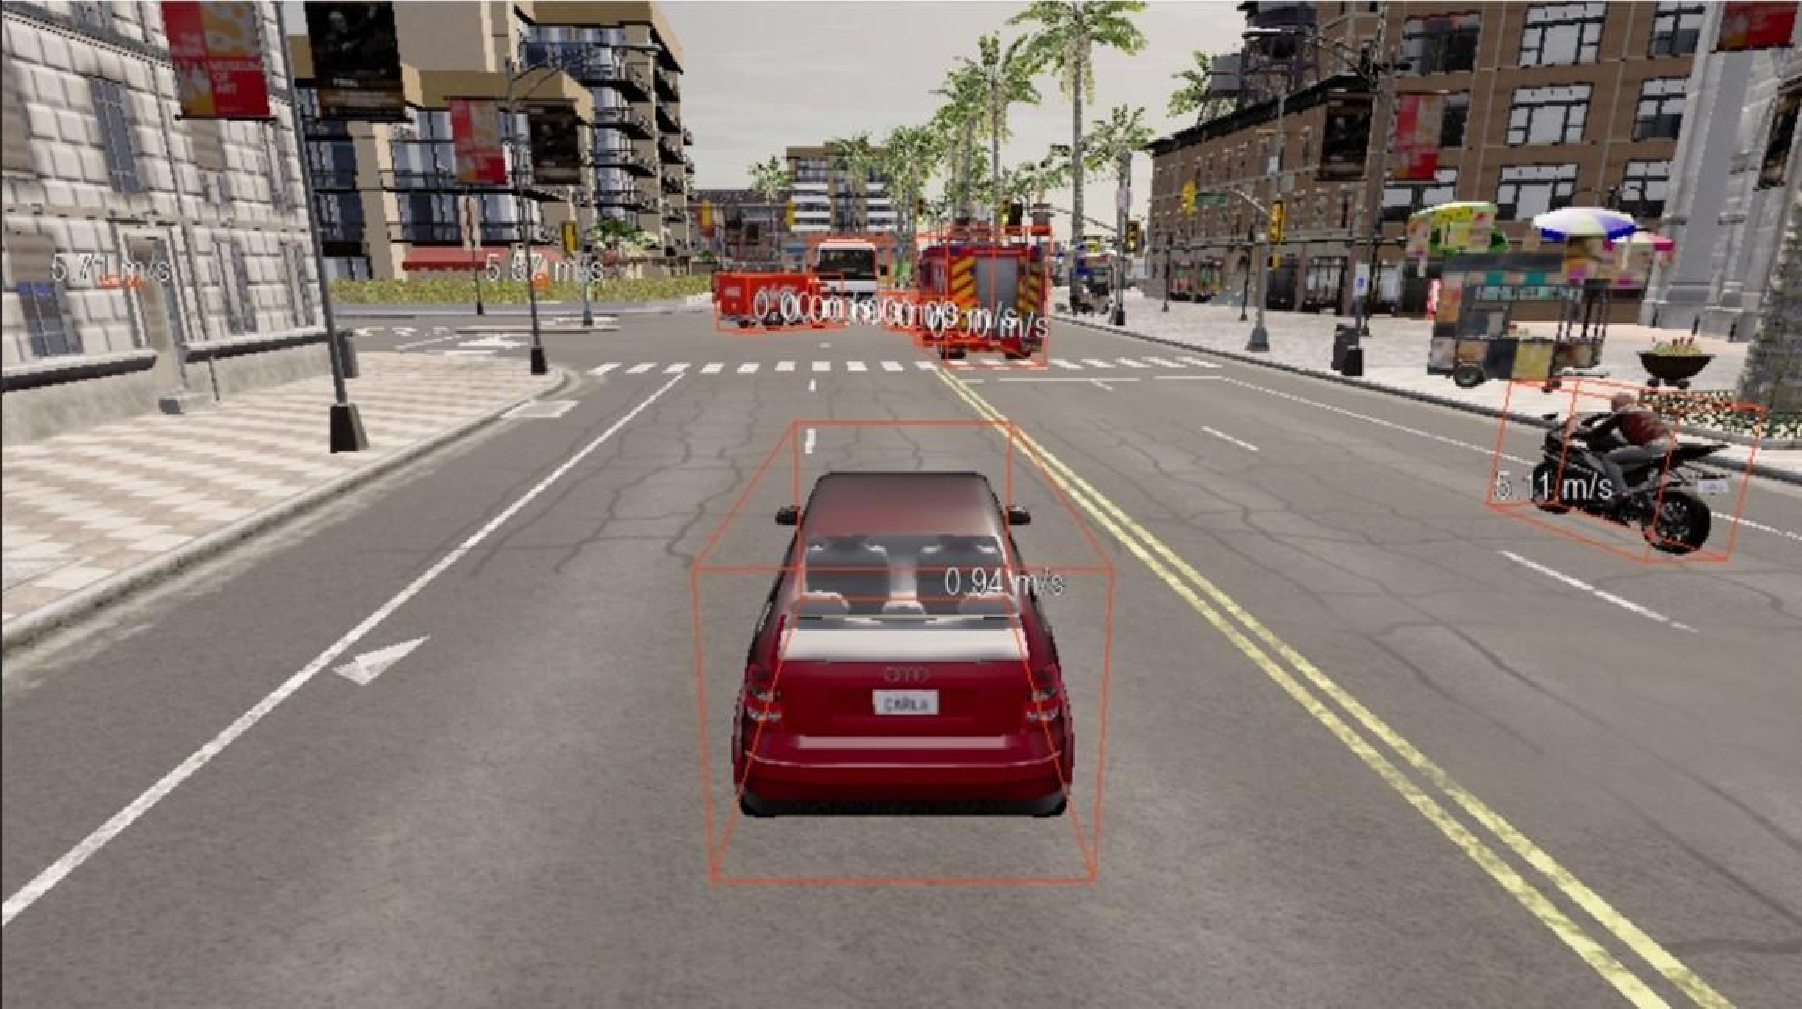
\includegraphics[width=0.8\textwidth]{images/图9 Bounding Box目标检测边界框示图.pdf}  % 引用转换后的 PDF 文件
    \caption{Bounding Box目标检测边界框示图}
    \label{fig:example_image}  % 可用于引用此图片
\end{figure}

该检测策略具有诸多优势。首先,精度高且完全依赖仿真物理参数,避免了检测误差与误判;其次,运算效率极高,检测过程不涉及卷积操作或复杂特征提取,极大减轻了系统负担;并且它的检测结果具备丰富的语义信息,如目标速度、加速度、位置与朝向等物理属性,为后续的行为分析提供了数据基础。此外,该方法可扩展性强,支持针对不同类别目标(如车辆、行人)进行个性化处理与标签生成,也可通过参数配置灵活控制采样频率与检测精度。

与基于神经网络的端到端检测方法(如 YOLO、Faster R-CNN 等)相比,本文采用的检测策略无需预训练模型与大规模样本集,显著降低了模型开发与部署门槛。同时,由于仿真环境的确定性与可控性,该方法具备良好的可复现性与一致性,适用于自动驾驶系统早期开发阶段的感知模块搭建、算法验证与功能测试等场景。

总体而言,本文设计的目标检测模块充分发挥了 Carla 平台在高保真仿真方面的优势,通过对三维边界框的几何建模与图像投影,构建了稳定、高效、可扩展的二维目标检测机制,为后续目标跟踪与意图识别模块提供了坚实的感知支撑。

\subsection{DeepSORT 跟踪模型集成}

目标跟踪的核心在于对同一目标在连续帧中的身份保持。在自动驾驶感知系统中,环境复杂、干扰因素多,目标可能因遮挡、加速、转弯等行为导致位置剧烈变化,因此构建一个稳定、高效的视觉跟踪机制至关重要。为此,本文基于 DeepSORT 算法构建了单目标实时跟踪模块,并将其集成至 Carla 仿真平台中的主控系统代码中,完成了从检测输入到轨迹输出的全流程功能。

与只依赖位置信息的传统方法相比,DeepSORT 在遮挡场景下仍具备较强的目标关联能力。本文使用的是 Python 社区中较为成熟的 deep\_sort\_realtime 版本,具有部署方便、接口清晰、适配灵活的特点。

在集成过程中,系统每帧将通过 Carla 投影方式生成的二维检测框(bounding box)作为 DeepSORT 的输入。检测结果先经过筛选(剔除面积过小、边界异常的框),再统一格式化为 [x, y, w, h] 的矩形框输入列表,与默认置信度、类别标签一起传入跟踪器。随后,DeepSORT 内部通过卡尔曼滤波器预测上一帧中所有跟踪目标的当前位置,并结合新一帧的检测框与历史轨迹,通过匈牙利算法完成目标匹配。在匹配过程中,除了利用 IOU(Intersection over Union)进行几何重叠度计算外,DeepSORT 还引入了由卷积神经网络提取的目标外观特征(ReID embedding),有效提升了在目标间相似度极高时的区分能力。

一旦目标匹配成功,系统会为其分配唯一的 Track ID,并持续更新其状态;当检测器识别出新目标且与现有轨迹无法匹配时,则自动分配新的 ID,形成新的跟踪轨迹。在本文系统中,由于为单目标跟踪设计,仅选取当前帧中距离自车最近的目标送入跟踪模块,从而保证跟踪的唯一性与稳定性。该策略不仅简化了系统复杂度,也便于后续意图分析模块聚焦处理单个危险对象。

为了实现视觉直观反馈,本文在每帧图像上使用 pygame 进行实时渲染,将当前追踪目标的边界框用醒目的黄色矩形高亮标出,如下图4-4所示,并在框上方以文字形式展示该目标的 Track ID。系统还通过颜色编码区分不同状态,如初始化、丢失、确认等,提升人机交互友好度。

\begin{figure}[H]
    \centering
    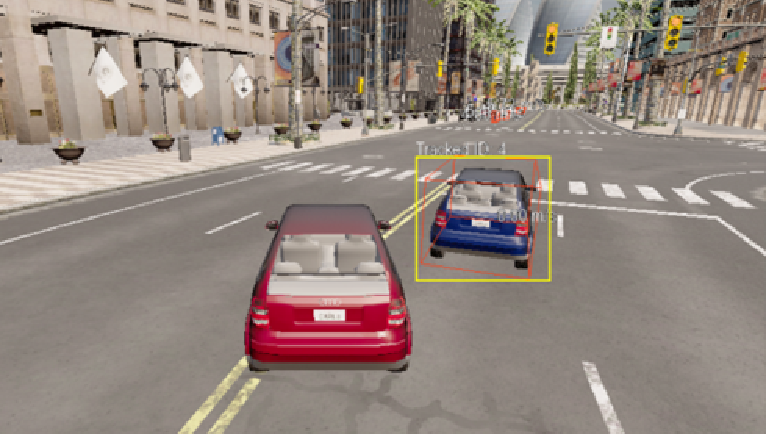
\includegraphics[width=0.8\textwidth]{images/图10 DeepSORT目标跟踪边界框示图.pdf}  % 引用转换后的 PDF 文件
    \caption{DeepSORT目标跟踪边界框示图}
    \label{fig:example_image}  % 可用于引用此图片
\end{figure}

整体来看,DeepSORT 模型在本系统中表现出良好的实时性与跟踪精度,尤其在交通场景中出现遮挡、快速移动等情况时仍能保持目标轨迹的连续性与身份一致性。该跟踪模块不仅为后续的行为意图分析提供了稳定的输入基础,也为系统未来拓展多目标跟踪或群体行为分析奠定了技术框架基础。

\section{模型性能评估}

为了系统性地评估本文所构建的视觉目标检测与跟踪模块的性能,实验从处理效率与运行稳定性两个维度展开。性能评估基于 Carla 仿真平台,在 Town10 和 Town01 等典型城市场景中进行,所有实验均在本地 Windows 平台(CPU:Intel i7-10750F,GPU:NVIDIA RTX 2060,内存 16GB)执行,未启用 GPU 加速推理,测试结果具备代表性。

\subsection{系统帧处理时序分析}

图 4-5 展示了系统处理一帧图像数据的完整流程及各阶段耗时情况,涵盖从仿真推进、图像获取、目标检测、目标跟踪、意图推理到用户界面渲染的全过程。为准确量化性能,各模块在主循环中添加了高精度计时器,记录时间戳并计算相邻阶段耗时,最终构建出帧处理的时序图。

\begin{figure}[H]
    \centering
    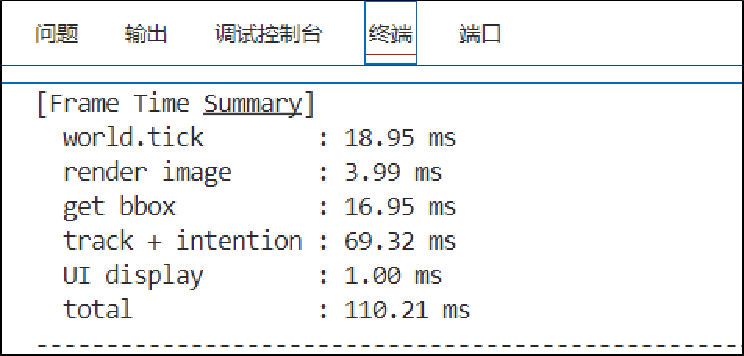
\includegraphics[width=0.8\textwidth]{images/图11 帧处理时序输出图.pdf}  % 引用转换后的 PDF 文件
    \caption{帧处理时序输出图}
    \label{fig:example_image}  % 可用于引用此图片
\end{figure}

将时序输出图转化成对应统计表格分析可知,单帧总处理时间为 110.21 毫秒,系统整体运行帧率约为 8.83 FPS,接近准实时运行性能要求。其中,各子模块平均耗时如下:

\begin{table}[htbp]
  \caption{模块时序统计表}
  \label{tab:timetable}
  \centering
  \begin{tabular}{lll}
    \toprule
    模块名称 & 平均耗时 & 比例估算 \\
    \midrule
    场景同步(tick) & 18.95ms & 17.2\% \\
    图像渲染(render) & 3.99ms & 3.6\% \\
    边界框生成(bbox) & 16.95ms & 15.4\% \\
    跟踪与意图分析 & 69.32ms & 62.9\% \\
    界面刷新(UI) & 1.00ms & 0.9\% \\
	总计(Total) & 110.21ms & 100\% \\
    \bottomrule
  \end{tabular}
\end{table}

场景同步(tick):平均耗时 5.98ms,主要用于与 Carla 仿真服务器同步并推进仿真世界一帧,属于系统的基础操作部分。耗时稳定,受仿真地图复杂度和传感器数量影响较小。

图像渲染(render):平均耗时 3.99ms,负责将图像传感器传回的原始 BGRA 数据解析为 RGB 格式,并转为 pygame 可渲染格式,供后续处理模块使用。该阶段性能稳定,是图像类任务的常规开销。

边界框生成(bbox):平均耗时 11.97ms,基于 Carla 内置的 3D Bounding Box 投影功能,从真实车辆模型构建顶点坐标并投影至摄像机图像平面。该方法替代了基于图像的传统目标检测网络,显著降低了计算开销,提升了标注精度,为后续跟踪提供了稳定输入。

跟踪与意图分析(track + intention):此模块耗时显著,高达 90.33ms,约占总帧处理时间的 80\%。主要包括 DeepSORT 的轨迹维护与状态更新(卡尔曼滤波、Hungarian 匹配、轨迹关联),以及基于目标运动状态的意图判别逻辑(距离变化率、速度阈值、接近风险判定等)。该阶段的高耗时是影响帧率的主要瓶颈,值得重点优化。

用户界面刷新(UI):平均耗时仅 1.00ms,主要用于文字信息与边界框在屏幕上的绘制,开销可忽略。

\subsection{模块耗时对比分析}

为进一步明确各模块在资源占用方面的相对贡献,本文将连续 100 帧的平均耗时统计结果绘制为柱状图(图 4-6)。可见,DeepSORT 跟踪模块与意图推理阶段占比最大,说明在今后的优化工作中,应首先考虑对该模块进行算法加速或模型压缩。

\begin{figure}[H]
    \centering
    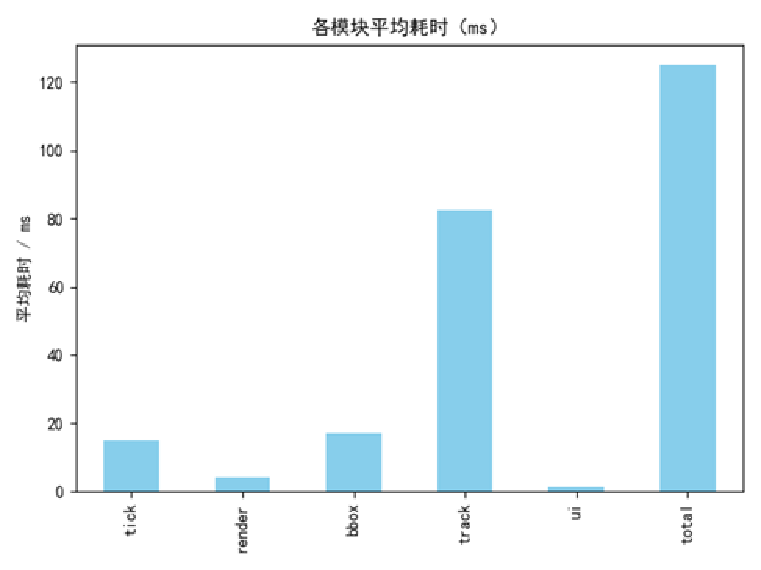
\includegraphics[width=0.8\textwidth]{images/图12 耗时统计柱状图.pdf}  % 引用转换后的 PDF 文件
    \caption{耗时统计柱状图}
    \label{fig:example_image}  % 可用于引用此图片
\end{figure}

可见,图像渲染与边界框生成等模块耗时较低,说明使用 Carla 平台原生的三维 bounding box 机制替代图像检测模型是一种有效的策略,不仅保证了高精度检测输入,同时大幅降低了计算资源占用。界面渲染部分耗时极少,可在后续部署时通过关闭 UI 进一步释放处理能力。


\begin{tabular}{l l}
%  \verb|\songti| & {\songti 宋体} \\
%  \verb|\heiti| & {\heiti 黑体} \\
%   \verb|\kaiti| & {\kaiti 楷体}
\end{tabular}
